\documentclass{ieeeaccess}

\usepackage[nocompress]{cite}
\usepackage{amsmath,amssymb,amsfonts}
\usepackage{graphicx}
\usepackage{textcomp}
\usepackage{booktabs}
\usepackage{tabularx}
\usepackage{array}
\usepackage{threeparttable}
\usepackage{multirow}
\usepackage{xspace}
\usepackage{bm}
\usepackage{xurl}
\usepackage{etoolbox}
\usepackage[bookmarksopen=false]{hyperref}
\hypersetup{colorlinks=true,citecolor=blue,urlcolor=blue,linkcolor=blue,pdfborder={0 0 0}}
\hypersetup{pdftitle={Endpoint Definitions and Label Provenance in Honey-Bee Toxicity Benchmarking},pdfauthor={Yongye Huang, Runqing Liao, Zhining Wang}}

% Bold math fonts, as set in the official IEEE Access template.
\makeatletter
% Suppress the production DOI label until an identifier has been assigned.
\patchcmd{\@maketitle}{Digital Object Identifier\space\@doi}{\ifx\@doi\@empty\else Digital Object Identifier\space\@doi\fi}{}{\PackageError{manuscript}{Unable to suppress an empty DOI field}{Check the IEEE Access title macro.}}
\AtBeginDocument{\DeclareMathVersion{bold}
\SetSymbolFont{operators}{bold}{T1}{times}{b}{n}
\SetSymbolFont{NewLetters}{bold}{T1}{times}{b}{it}
\SetMathAlphabet{\mathrm}{bold}{T1}{times}{b}{n}
\SetMathAlphabet{\mathit}{bold}{T1}{times}{b}{it}
\SetMathAlphabet{\mathbf}{bold}{T1}{times}{b}{n}
\SetMathAlphabet{\mathtt}{bold}{OT1}{pcr}{b}{n}
\SetSymbolFont{symbols}{bold}{OMS}{cmsy}{b}{n}
\renewcommand\boldmath{\@nomath\boldmath\mathversion{bold}}}

% IEEE reference style: list all authors through six, then first author et al.
\newcommand{\applyIEEEbibcontrol}{\if@filesw
  \immediate\write\@auxout{\string\citation{IEEEControl}}\fi}
\makeatother

% Measurement and metric macros.
\newcommand{\ugbee}{\ensuremath{\mu\mathrm{g\,bee}^{-1}}\xspace}
\newcommand{\auroc}{\mathrm{AUROC}}
\newcommand{\ap}{\mathrm{AP}}
\newcommand{\ldfifty}{\mathrm{LD}_{50}}

\newcolumntype{Y}{>{\raggedright\arraybackslash}X}
\newcolumntype{C}{>{\centering\arraybackslash}X}

% Lets TeX stretch interword space in the narrow two-column measure
% instead of overrunning the margin.
\setlength{\emergencystretch}{1.5em}

% Keep at least two paragraph lines together at column and page breaks.
\clubpenalty=10000
\widowpenalty=10000
\displaywidowpenalty=10000

\begin{document}
\raggedbottom
\applyIEEEbibcontrol

\history{}
\doi{}

\title{Endpoint Definitions and Label Provenance in Honey-Bee Toxicity Benchmarking}

\author{\uppercase{Yongye Huang}\authorrefmark{1},
\uppercase{Runqing Liao}\authorrefmark{1},
AND \uppercase{Zhining Wang}\authorrefmark{1}}

\address[1]{School of Mathematics and Statistics, Hanshan Normal University, Chaozhou 521041, China (e-mail: hiiy132321@163.com; 202411055222@stu.hstc.edu.cn; mathwangzhining@163.com)}

\tfootnote{This work was supported by the National Natural Science Foundation of China under Grant 12671554 and by the Department of Education of Guangdong Province, China, under Grant 2024ZDZX1027.}

\markboth
{Huang \headeretal: Endpoint Definitions and Label Provenance in Honey-Bee Toxicity Benchmarking}
{Huang \headeretal: Endpoint Definitions and Label Provenance in Honey-Bee Toxicity Benchmarking}

\corresp{Corresponding author: Zhining Wang (e-mail: mathwangzhining@163.com).}

\begin{abstract}
Toxicity benchmarks encode both endpoint thresholds and the rules used to combine experimental records. We developed a retrospective audit of ApisTox that connects endpoint discrimination to historical label construction and tests the predictive consequences of traceable label revisions. On the same 1,035 compounds and official splits, the 100-microgram-per-bee endpoint had the lowest area under the receiver operating characteristic curve (AUROC) in all 15 representation--split settings. Circular-fingerprint AUROCs on the structure-diverse split were 0.592, 0.792 and 0.795 at thresholds of 100, 11 and 1 micrograms per bee. Tier-pair decomposition localized the deficit to comparisons between compounds annotated at (11,100] and above 100. Upstream-code replay reproduced all 441 Ecotoxicology Knowledgebase (ECOTOX)-derived annotations and confirmed loss of inequality qualifiers. A four-rule audit separated qualifier handling from aggregation; among 212 ECOTOX-derived compounds annotated at (11,100], qualifier-aware consensus on the historical determining routes yielded 32 positive, 67 negative and 113 unresolved labels at 100. A separate matched-cohort crossover of original and provisionally revised labels showed no consistent narrowing of the endpoint gap under the primary revision scenario. With unresolved labels retained, the structure-diverse 11-minus-100 gap changed from 0.200 to 0.234 (change 0.034; conditional 95\% confidence interval $-0.040$ to 0.113). The audit distinguishes reproducible annotation defects from their predictive consequences and provides a record-to-evaluation workflow for examining toxicity benchmarks.
\end{abstract}

\begin{keywords}
Benchmarking, data quality, endpoint definition, honey bee, label noise, machine learning, regulatory toxicology, structure--activity relationship.
\end{keywords}

\titlepgskip=-21pt

\maketitle

\section{Introduction}
\label{sec:introduction}
\PARstart{P}{redictive} models of honey-bee toxicity support chemical screening and pesticide assessment. Their evaluation depends on a defined prediction target as well as a suitable representation and learner. For \textit{Apis mellifera}, whose pollination supports agriculture and ecosystem functioning\cite{Patel2021}, acute toxicity is commonly expressed through dose-based mortality endpoints. The Organisation for Economic Co-operation and Development (OECD) identifies a defined endpoint, an unambiguous algorithm, an applicability domain and adequate performance assessment as central elements of regulatory quantitative structure--activity relationship (QSAR) evaluation\cite{OECD2014,OECD2023}.

ApisTox provides a shared resource of 1,035 compounds with predefined Random, MaxMin and Time splits\cite{Adamczyk2025}, and recent studies use it to compare learning architectures and molecular representations\cite{Adamczyk2026,Damiao2025,Pinho2026,Adamczyk2025b}. Its native binary task labels 296 compounds as toxic at 11~\ugbee. The benchmark also distributes a three-level annotation with cut-offs at 1 and 100~\ugbee, so the same compounds support nested endpoints at 100, 11 and 1~\ugbee. Other honey-bee models use the 100~\ugbee cut-off\cite{Iovine2026}. The resulting tasks differ in positive-class membership and the source annotations that determine it.

Endpoint comparisons hold molecular representations fixed while changing class prevalence and the chemical composition of each class. Performance differences can therefore reflect both the prediction task and how its labels were constructed. Previous QSAR studies have compared alternative thresholds on a fixed compound set as well as after excluding intermediate compounds\cite{Wang2023}; dataset definitions are central to the resulting model claim\cite{Nael2026}. We ask which tier comparisons underlie the ApisTox endpoint gap and whether the released labels preserve source-record qualifiers. We then test whether provisional revisions supported by accessible records reduce that gap.

We connect paired endpoint evaluation to the historical transformations that produced the released labels. The analysis measures the area under the receiver operating characteristic curve (AUROC), locates the contributing tier comparisons, and tests how source-supported revisions change the measured gap. The study makes three contributions:
\begin{enumerate}
\setlength{\itemsep}{1pt}
\item \textbf{Controlled endpoint comparison and localization.} Common compounds, official splits and fixed learner specifications expose the broad-endpoint deficit; tier-pair decomposition identifies the weakly ranked comparisons that dominate it.
\item \textbf{Record-to-label reconstruction.} Replication of the ECOTOX pipeline reproduces the released annotations, identifies qualifier loss, and separates its label effects from those of aggregation choices.
\item \textbf{Matched-cohort revision testing.} A training-by-evaluation crossover distinguishes changes to fitting labels from changes to evaluation labels and measures whether traceable revisions narrow the endpoint gap.
\end{enumerate}
Fig.~\ref{fig:design} outlines the design.

\begin{figure*}[!t]
\centering
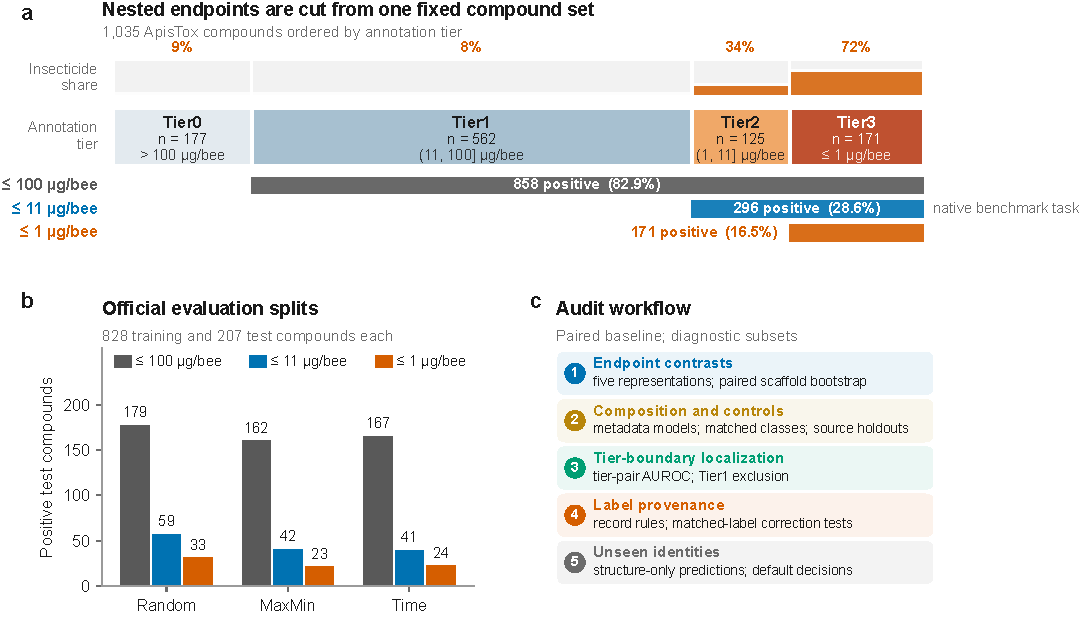
\includegraphics[width=\linewidth]{Fig1_study_design.pdf}
\caption{\textbf{Study design.} \textbf{(a)} The three nested benchmark-derived toxicity endpoints drawn on the fixed set of 1,035 compounds ordered by severity tier. Bar widths are proportional to tier size, and the strip above reports the insecticide share of each tier. The 11~\ugbee endpoint reproduces the native binary task distributed with the benchmark. \textbf{(b)} Positive compounds in each official 207-compound test set. \textbf{(c)} The five analysis stages. The primary endpoint comparison uses common compounds, splits and learner specifications; later diagnostic and source-based stages include explicitly defined subsets.}
\label{fig:design}
\end{figure*}

\section{Related Work}
\label{sec:related}
\subsection{Honey-bee toxicity prediction}
Honey-bee toxicity modelling includes descriptor and fingerprint classifiers, mode-of-action profiling and prediction tools\cite{Venko2018,Carnesecchi2020,Xu2021,MoreiraFilho2021}. Recent ApisTox studies compare graph neural networks, transfer learning and classical representations\cite{Adamczyk2026,Damiao2025,Pinho2026,Adamczyk2025b}; BeeEcoTox integrates source data for graph-based prediction\cite{Chen2026}.

Data-curation choices define the prediction targets in these studies. Carnesecchi et al.\cite{Carnesecchi2020} screened adult 48-hour contact records and handled conflicting observations. Iovine et al.\cite{Iovine2026} developed an oral-toxicity classifier with duplicate-record rules that distinguish exact values from lower bounds. Both studies used \(<100\) versus \(\geq100\)~\ugbee, placing equality on the opposite side from the released annotations audited here. We examine the processing history of the released benchmark itself, then test how alternative record-to-label rules affect evaluation on matched cohorts.

\subsection{Benchmark labels and label noise}
Label noise degrades classifier performance and complicates its assessment\cite{Frenay2014}; test-set errors can also change model rankings\cite{Northcutt2021}. Molecular benchmarks depend on curation, metrics and split design\cite{Wu2018}, and time-split validation has been proposed to approximate prospective prediction\cite{Sheridan2013}. Wang et al.\cite{Wang2023} compared thresholds on a fixed compound set and after removing intermediate compounds. Nael et al.\cite{Nael2026} argued for executable dataset contracts with explicit endpoint and aggregation rules. Our record-level replay and matched-cohort crossover connect these two questions: which processing choices alter the labels, and how those revisions alter the observed endpoint comparison.

\subsection{Experimental variability and censored toxicity values}
Experimental uncertainty limits the performance that any model can achieve on public activity data\cite{Brown2009,Kramer2012}, and replicate acute oral median lethal dose (LD\(_{50}\)) studies in rats vary substantially\cite{Karmaus2022}. Acute honey-bee tests add a design feature: when a limit test at 100~\ugbee shows that the LD\(_{50}\) exceeds that dose, the result is reported as \(>100\)~\ugbee\cite{OECD213,OECD214}. Their reported lower bounds coincide with the broad cut-off studied here. Svensson et al.\cite{Svensson2025} incorporated censored assay labels into regression models for predictive uncertainty quantification in drug discovery. Our retrospective audit reconstructs how censoring and aggregation rules shape released categorical benchmark labels, then tests the predictive consequences of traceable revisions.

\section{Materials and Methods}
\subsection{Dataset and endpoint construction}
We used the ApisTox v2 dataset of 1,035 compounds with valid simplified molecular-input line-entry system (SMILES) representations and toxicity annotations\cite{Adamczyk2025}. Recorded sources were the Pesticide Properties Database (PPDB; 510)\cite{Lewis2016}, the Ecotoxicology Knowledgebase (ECOTOX; 441) and the Biopesticides Database (BPDB; 84). Each compound also carried an exposure-type field (Contact, Oral or Other) and four non-mutually exclusive chemical-use flags; 55 records had no use flag.

The benchmark distributes a binary annotation at 11~\ugbee and a ternary annotation with boundaries at 1 and 100~\ugbee\cite{Adamczyk2025}. In its ECOTOX pipeline, route-specific record groups spanning both sides of 11 are removed, the binary label is assigned from the remaining group's numerical range, and the ternary level is assigned from its median. The compound inherits the eligible route with the lowest median. The binary code includes an equality convention at 11 detailed in Supplementary Methods. The two annotations therefore encode different aggregation rules. Their combination defines four analytical tiers, Tier0--Tier3 (Table~\ref{tab:endpoints}), whose ranges summarize the released annotations. Writing the tier of compound \(i\) as \(g_i\in\{0,1,2,3\}\), the endpoint labels are
\begin{equation}
y_i^{(\tau)}=\mathbf{1}\{g_i\geq k_\tau\},\qquad
(k_{100},k_{11},k_1)=(1,2,3).
\label{eq:endpoint-map}
\end{equation}
We call the 100~\ugbee endpoint the broad endpoint and the 11 and 1~\ugbee endpoints the severe endpoints. These are operational prediction targets; the source category ``non-toxic'' means benchmark-negative at its cut-off, not safety under other exposures or outcomes. The 11~\ugbee endpoint reproduces the native benchmark task. We kept the distributed annotations for the benchmark comparison and audited numerical values, qualifiers and exclusion records separately (Section~\ref{sec:provenance-methods}).

\begin{table*}[!t]
	\centering
	\caption{\textbf{Construction and prevalence of the nested benchmark endpoints.}}
	\label{tab:endpoints}

	\begin{minipage}{0.90\linewidth}
		\centering

		\begin{tabular}{@{}l p{0.38\linewidth} p{0.23\linewidth} r@{}}
			\toprule
			\multicolumn{4}{c}{\textbf{a. Analytical tier construction}} \\
			\midrule
			\textbf{Tier} &
			\textbf{Benchmark annotation} &
			\textbf{Annotation-implied range} &
			$\boldsymbol{n}$ \\
			\midrule
			Tier0 & Ternary level non-toxic & \(>100~\ugbee\) & 177 \\
			Tier1 & Ternary level moderate, binary label non-toxic & \((11,100]~\ugbee\) & 562 \\
			Tier2 & Ternary level moderate, binary label toxic & \((1,11]~\ugbee\) & 125 \\
			Tier3 & Ternary level highly toxic & \(\leq1~\ugbee\) & 171 \\
			\bottomrule
		\end{tabular}

		\vspace{0.9em}

		\begin{tabular}{@{}lrrrr@{}}
			\toprule
			\multicolumn{5}{c}{\textbf{b. Positive compounds in the official test sets}} \\
			\midrule
			\textbf{Split} &
			\textbf{Test} $\boldsymbol{n}$ &
			\textbf{100~\ugbee} &
			\textbf{11~\ugbee} &
			\textbf{1~\ugbee} \\
			\midrule
			Random & 207 & 179 (86.5\%) & 59 (28.5\%) & 33 (15.9\%) \\
			MaxMin & 207 & 162 (78.3\%) & 42 (20.3\%) & 23 (11.1\%) \\
			Time & 207 & 167 (80.7\%) & 41 (19.8\%) & 24 (11.6\%) \\
			\bottomrule
		\end{tabular}

		\vspace{0.5em}

		\footnotesize
		\raggedright
		\textit{Note.}
		The binary label uses the U.S. Environmental Protection Agency (EPA) threshold (toxic at or below 11~\ugbee) and the ternary level uses the PPDB thresholds (1 and 100~\ugbee); the benchmark applies both to records from all three source databases. Endpoint columns report the number and proportion of positive test compounds at or below the indicated cut-off. The Time split uses a PubChem literature-date proxy with compound-record creation dates as a fallback.

	\end{minipage}
\end{table*}

\subsection{Evaluation splits and leakage control}
We used the official ApisTox Random, MaxMin and Time splits with the compound membership distributed in the Zenodo release\cite{Adamczyk2025}. Each split contains 828 training and 207 test compounds. Random approximates interpolation under random sampling. MaxMin provides a structurally diverse within-dataset holdout. Time uses the benchmark's PubChem literature-date proxy, with compound-record creation dates as a fallback\cite{Adamczyk2025}; these dates do not identify when the toxicity experiments were performed. Within each fit, scaling, hyperparameter selection, calibration, feature selection and fusion used training data only. The same benchmark and official test sets had been inspected during earlier exploratory modelling; the present study is a retrospective evaluation.

\subsection{Molecular representations and fixed learners}
We evaluated five molecular representations. The binary fingerprints were extended-connectivity fingerprints (ECFP; ECFP4/Morgan, radius 2, 1,024 bits)\cite{Rogers2010}, 1,024-bit Avalon fingerprints\cite{Gedeck2006} and Molecular Access System (MACCS) keys\cite{Durant2002}. The Weisfeiler--Lehman subtree representation with histogram intersection (WL-HI)\cite{Shervashidze2011} used atom labels combining element, formal charge and aromaticity, together with bond-typed neighbourhoods. Two refinement iterations were followed by histogram-intersection feature expansion and cosine normalization. The 12 physicochemical descriptors were molecular weight, logP, topological polar surface area, hydrogen-bond donors and acceptors, rotatable bonds, ring count, aromatic ring count, fraction sp\textsuperscript{3}, heavy-atom count, molar refractivity and formal charge. A robust scaler was fitted to the training descriptors.

Binary fingerprints were compared using the Tanimoto kernel
\begin{equation}
K_T(x_i,x_j)=\frac{x_i^\top x_j}{\lVert x_i\rVert_1+\lVert x_j\rVert_1-x_i^\top x_j}.\label{eq:tanimoto}
\end{equation}
Structure models used class-weight-balanced support-vector machines (SVMs)\cite{Cortes1995} with a precomputed kernel and regularization parameter \(C=1\). The descriptor model used a radial basis function (RBF) kernel with \(C=1\) and scale-adjusted \(\gamma\). ECFP was the primary representation, and the other representations assessed robustness. Learner specifications and preprocessing protocols were held constant across endpoints within each analysis; balanced class weights varied with endpoint prevalence.

Learner sensitivities used ECFP4 bit vectors with L2-regularized logistic regression and a 500-tree random forest. Logistic-regression \(C\) was selected from \(\{0.01,0.1,1,10\}\) by five-fold training-set cross-validation using AUROC; the random forest used balanced-subsample class weights. Supplementary Table~S21a provides the complete configurations. Analyses used RDKit 2025.09.4\cite{RDKit2025_09_4} and scikit-learn 1.8.0\cite{Pedregosa2011}, with root seed 20260829. Supplementary Methods define the class-weighted objective and WL-HI feature map, and Supplementary Algorithm S1 summarizes the paired evaluation.

For probability analyses, five-fold stratified out-of-fold decision scores from the training set were used to fit a Platt sigmoid\cite{Platt1999}. The fitted calibrator was applied to test decision scores.

\subsection{Evaluation metrics and paired uncertainty}
The primary metric was the AUROC, the probability that a positive compound outranks a negative compound, with half credit for tied scores. Let \(s_i^{(a)}\) be the held-out score from the model trained for endpoint \(a\). On one test set, define \(\mathcal P_b=\{i:y_i^{(b)}=1\}\), \(\mathcal N_b=\{i:y_i^{(b)}=0\}\) and their sizes \(n_b^+\) and \(n_b^-\). With \(h(u,v)=\mathbf1\{u>v\}+\tfrac12\mathbf1\{u=v\}\),
\begin{equation}
\widehat A_{a\to b}=\frac{1}{n_b^+n_b^-}
\sum_{i\in\mathcal P_b}\sum_{j\in\mathcal N_b}
h\!\left(s_i^{(a)},s_j^{(a)}\right).
\label{eq:paired-auc}
\end{equation}
Diagonal entries quantify endpoint-specific discrimination; off-diagonal entries evaluate the same learned ranking against another endpoint's labels. Grouping the positive--negative pairs in \eqref{eq:paired-auc} by tier gives
\begin{equation}
\widehat A_{a\to b}=\sum_{r=k_b}^{3}\sum_{\ell=0}^{k_b-1}
w_{r\ell}^{(b)}\,\widehat q_{r\ell}^{(a)},\qquad
w_{r\ell}^{(b)}=\frac{n_rn_\ell}{n_b^+n_b^-},
\label{eq:tier-pair}
\end{equation}
where \(n_r\) counts test compounds in Tier \(r\) and the tier-pair AUROC \(\widehat q_{r\ell}^{(a)}\) is the probability that a Tier~\(r\) compound outranks a Tier~\(\ell\) compound under the scores of model \(a\) (Supplementary Methods). The weights depend only on the test-set tier counts, so an endpoint dominated by poorly separated tier pairs has a low AUROC even when its other pairs are ranked well. AUROC is undefined when either class is absent. Average precision was reported only within endpoints because its random baseline equals endpoint prevalence. Probabilistic prediction error was assessed with the Brier score\cite{Brier1950} and expressed as Brier skill relative to a constant forecast equal to the training-set prevalence.

Two severe-minus-broad contrasts were designated as primary for reporting at the analysis freeze: \(\widehat\Delta_b=\widehat A_{b\to b}-\widehat A_{100\to100}\), for \(b\in\{11,1\}\). We drew 5,000 paired bootstrap samples, reusing the same resampled test indices across endpoints. A second bootstrap sampled Bemis--Murcko scaffolds\cite{Bemis1996} as clusters, with acyclic compounds retained as distinct structure units. Simultaneous 95\% confidence intervals (CIs) used the joint centred bootstrap distribution of the two primary contrasts within each split and resampling level.

Bootstrap intervals describe empirical reweighting variability within each evaluated test cohort, conditional on the training data, fitted models, label rules, split assignments and analysis protocol. Training, label-adjudication and analysis-selection uncertainty lie outside this conditional estimate. A multiplicity sensitivity widened the family to ten contrasts across five representations within each split, using the same replicates. Overlapping test compounds and shared labels make the settings dependent, so counts of positive contrasts summarize consistency across settings. Cross-endpoint AUROC intervals used 2,000 scaffold-cluster replicates.

\subsection{Tier-boundary analyses}
\label{sec:tier-methods}
Tier-pair AUROCs were computed from the saved held-out scores of every representation and training endpoint, with scaffold-cluster percentile intervals over the primary bootstrap draws. Tier1 exclusion then removed the Tier1 compounds, first from the test set only and then from both training and test sets, where the same fixed learner was refitted to separate Tier0 from Tier2 and Tier3. Without Tier1, the two cut-offs define the same labels on the reduced set; the all-tier 11~\ugbee reference still uses its original train/test members. The severe-minus-broad gap therefore decomposes exactly as
\begin{equation}
\begin{aligned}
\widehat A_{11\to11}-\widehat A_{100\to100}
={}&\bigl[\widehat A^{-1}_{100}-\widehat A_{100\to100}\bigr]\\
&+\bigl[\widehat A^{-1}_{\mathrm{refit}}-\widehat A^{-1}_{100}\bigr]\\
&+\bigl[\widehat A_{11\to11}-\widehat A^{-1}_{\mathrm{refit}}\bigr],
\end{aligned}
\label{eq:tier1-decomposition}
\end{equation}
where \(\widehat A^{-1}_{100}\) evaluates the original broad model on the Tier1-free test set and \(\widehat A^{-1}_{\mathrm{refit}}\) evaluates the refitted model on the same set. The first two terms form the Tier1 component and the last term is the residual. Intervals use the scaffold-cluster draws of the primary analysis, so they are paired with the primary contrasts. Removing Tier1 changes the evaluation pairs, training members and class weights. The component is a descriptive deletion contrast.

\subsection{Composition analysis and model decomposition}
Associations between Tier and source, route or use flags were summarized with contingency tables, chi-squared tests and Cram\'{e}r's \(V\). Benjamini--Hochberg false discovery rate (BH-FDR) correction was applied within the metadata family of six association tests (source, route and the four use indicators; Supplementary Table~S21b)\cite{Benjamini1995}.

We compared five predictive specifications. The source-plus-route model contained only the source database and exposure route. The agrochemical-use model contained the four use indicators, and the all-metadata model contained the use indicators, source and exposure route. These three models used training-fitted one-hot encoding and an L2-regularized logistic classifier with class weighting. The structure model was the fixed ECFP/Tanimoto SVM. For structure-plus-metadata fusion, five-fold out-of-fold ECFP decision scores were generated in the training set and combined with metadata in a second-stage logistic model. The ECFP model was then refitted to all training compounds, and its test score was supplied to the fitted second-stage model. This procedure prevented the fusion layer from observing in-sample structural scores or test labels. Metadata-only and fused models were additionally refitted with identical standardization of all inputs, with and without the exposure-type field. This is a point-estimate sensitivity; intervals refer to the original decomposition protocol.

\subsection{Matched-class learning curves and source holdouts}
To evaluate whether different class counts explained endpoint ordering, we sampled equal numbers of positive and negative training compounds at 25, 50, 75, 100 and 125 per class. Each sample size was repeated 200 times with the fixed ECFP learner and evaluated on the unchanged official test set. Quantile bands summarize variability across repeated training subsamples conditional on the official test set. In leave-one-source-out analyses, models were fitted to compounds from the remaining source databases and evaluated on the held-out source. These holdouts assess sensitivity to the recorded source under the shared benchmark label mapping.

\subsection{Regulatory-source reassessment and qualifier tracing}
\label{sec:provenance-methods}
OpenFoodTox 3.0 v7 and the EPA retrospective S1--S5 tables\cite{OFT2026,Farruggia2022} supplied acute \textit{A.~mellifera} LD\(_{50}\) observations. Alignment used the hashed International Chemical Identifier (InChIKey), connectivity checks and source-identity review. The OpenFoodTox screen excluded known metiram/zineb representation conflicts and inconsistent International Chemical Identifier (InChI)/SMILES records. EPA source-structure discrepancies were retained in broad analyses and excluded in the stated structure and study-identifier sensitivity screen. Numerical units and inequality qualifiers were preserved: \(>100\) gives a negative 100~\ugbee label, whereas \(\geq100\) leaves it unresolved. Assigned labels required all selected observations to agree on one side of each cut-off. Concordance with the benchmark was assessed on same-route cohorts with all three labels determined and was tabulated by benchmark tier and by benchmark record source, with Wilson 95\% intervals for agreement rates.

The upstream ApisTox code\cite{ApisToxCode} omits ECOTOX response operators and removes leading inequality signs from PPDB/BPDB values. We reproduced the binary label, ternary level and determining route of all 441 ECOTOX-derived benchmark compounds, enforced by assertions.

At each of the three cut-offs, a factorial audit compared (A) numerical medians with operators ignored, (B) numerical all-record consensus, (C) qualifier-aware all-record consensus and (D) the feasible interval of the median. Consensus is determinate only when every retained record is determinate and agrees. Rule D compares the median's interval with the threshold.

We separately evaluated the original determining route, the minimum over upstream-eligible routes and the minimum over all routes. A minimum is positive if any route is determinately positive and negative only if every available route is determinately negative; this need not identify a unique corrected determining route. Record filters retained all upstream-accepted observations, adult 48-hour non-daily-dose observations, or their active-ingredient subset. Empty filtered groups were distinguished from unresolved groups (Supplementary Table~S22). The PPDB/BPDB input snapshots used to construct the benchmark were unavailable, preventing reconstruction of their individual parser effects.

The retrospective cross-source reassessment paired saved held-out scores with source-derived contact labels, excluding each model's training identities and using a common three-cut-off cohort. Broad cohorts included original mixed-route labels; stricter cohorts required original contact labels. The OpenFoodTox screen additionally required 48-hour observations and excluded material-review flags and explicit test-material dose reports. The EPA screen required structure consistency and master record identification (MRID) evidence. For records with missing material fields, active-ingredient status remained unverified.

For the primary ECFP model, 5,000 paired compound draws evaluated contrasts and label-source changes. Classes below five compounds were flagged, single-class AUROC was undefined, and counts of valid and degenerate draws were retained; percentile intervals used jointly valid draws only. This phase was designed after source-label inspection. The sources may share underlying studies, including EPA records also accessible through ECOTOX\cite{Farruggia2022}. For a common eligible cohort, let \(\widehat A^{(L)}_{a\to b}\) denote \eqref{eq:paired-auc} evaluated using label source \(L\). The source-label change in each primary contrast is
\begin{equation}
\begin{aligned}
\widehat\Gamma_b&=\widehat\Delta_b^{(\mathrm{source})}
-\widehat\Delta_b^{(\mathrm{benchmark})},\\
\widehat\Delta_b^{(L)}&=\widehat A^{(L)}_{b\to b}
-\widehat A^{(L)}_{100\to100}.
\end{aligned}
\label{eq:source-shift}
\end{equation}
The cohort and endpoint-specific score vectors are identical under the two label sources. Thus \(\widehat\Gamma_b\) measures sensitivity to the evaluation-label source, including changes in class membership and source aggregation.

\subsection{Training-by-evaluation label crossover}
We crossed original and provisionally revised training labels with original and provisionally revised evaluation labels. This retrospective sensitivity analysis was designed after inspecting endpoint performance and source-label discrepancies. The designated primary revision used rule D at 1 and 100~\ugbee and rule C at 11~\ugbee, taking the minimum over upstream-eligible ECOTOX routes. Sensitivities used consensus at all cut-offs, adult 48-hour non-daily-dose records, route-matched regulatory labels, or combined ECOTOX and regulatory evidence. Direct ECOTOX scenarios retained PPDB/BPDB labels; regulatory and combined scenarios could revise them when matched evidence existed. The resulting label sets therefore combined retained benchmark annotations with scenario-specific provisional revisions.

ECOTOX identities with no eligible filtered records entered the same handling policy as unresolved labels. In the regulatory scenario, identities without any matched source record retained their distributed labels. The handling policies retained unresolved labels at their original values, excluded affected identities at all cut-offs, or assigned negative only at 100~\ugbee as an extreme sensitivity assumption. The last assignment can produce a negative broad label with a positive severe label. We report it solely as a non-nested stress test and exclude it from correction inferences. Each of five scenarios and three handling rules was evaluated for five representations and three splits: 225 settings comprising 150 nested correction settings and 75 non-nested stress-test settings, each with both severe-minus-broad contrasts (Supplementary Table~S23).

Within each setting, all four cells used identical training and test identities. Full-cohort original-label fits reproduced saved scores within \(10^{-9}\); after exclusion, both training-label versions were refitted on the same retained members. Scaling and class weights were re-estimated within each fit. Each split/cohort used 2,000 shared scaffold-cluster bootstrap draws to estimate percentile intervals for AUROC, each gap and its change. These exploratory intervals describe reweighting variability in each evaluated cohort, conditional on fitted models, label rules and the analysis protocol. They are not multiplicity-adjusted across correction scenarios; exclusion scenarios target a selected cohort. Per-compound scores, membership hashes, class counts and valid-draw counts accompany the results.

\subsection{Case study on unseen chemical identities}
The supplementary case study screened sixteen recently introduced pesticide active ingredients. Two benchmark overlaps were excluded by connectivity; ten structures were predicted, and six supplied eligible 48-hour adult endpoints. The initial eight structures were fixed before inference. The two additional structures were frozen after their numerical toxicity endpoints and threshold labels had been curated; the prediction runner used structure-only inputs. The retained records do not establish whether outcomes were known at first nomination. Nine original ECFP models were restored without external outcomes, reproducing 1,863 saved scores within \(2.22\times10^{-16}\). Predictions used the balanced SVM's fixed zero-score boundary. The two-batch selection, record eligibility, restoration and all predictions are reported in Supplementary Methods and Tables~S19--S20.

\subsection{Secondary structural diagnostics}
Neighbourhood mixing tested with composition-conditional permutation, leave-one-out scaffold context, novelty-dependent calibration and nested sparse-descriptor selection are specified in Supplementary Methods. No test result selected a preferred descriptor subset size.

\subsection{Identifier and aggregation sensitivities}
We compared the frozen SMILES with current PubChem structures for every stored compound identifier (CID), using responses retrieved on 3 October 2026\cite{PubChem2025}. Complete InChIKey, connectivity-block and standardized fragment-parent comparisons defined an identifier-consistency screen. Identities lacking a direct connectivity match formed a fixed screening set, recorded before its predictive evaluation. We retained the official splits and excluded these identities from both training and test partitions, then refitted the ECFP models with the original settings. Evaluation of the saved original models on the same reduced test members separated test-composition from refitting changes. Paired scaffold-cluster intervals used 5,000 draws, with simultaneous intervals for the two endpoint contrasts within each split and evaluation stage. This screen neither replaces historical structures nor establishes a label-error rate (Supplementary Table~S26).

A second sensitivity applied interval-median rule D at all three cut-offs. We compared final labels under the keep policy and refitted the matched-member ECFP crossovers under exclude where training inputs changed. A separate replay assessed a documented source-report qualifier discrepancy without modifying the archived export. Supplementary Methods and Table~S25 document these checks, the exact historical equality convention and the distinction between exclusion-log scope and executed filtering.

\begin{figure*}[!t]
	\centering
	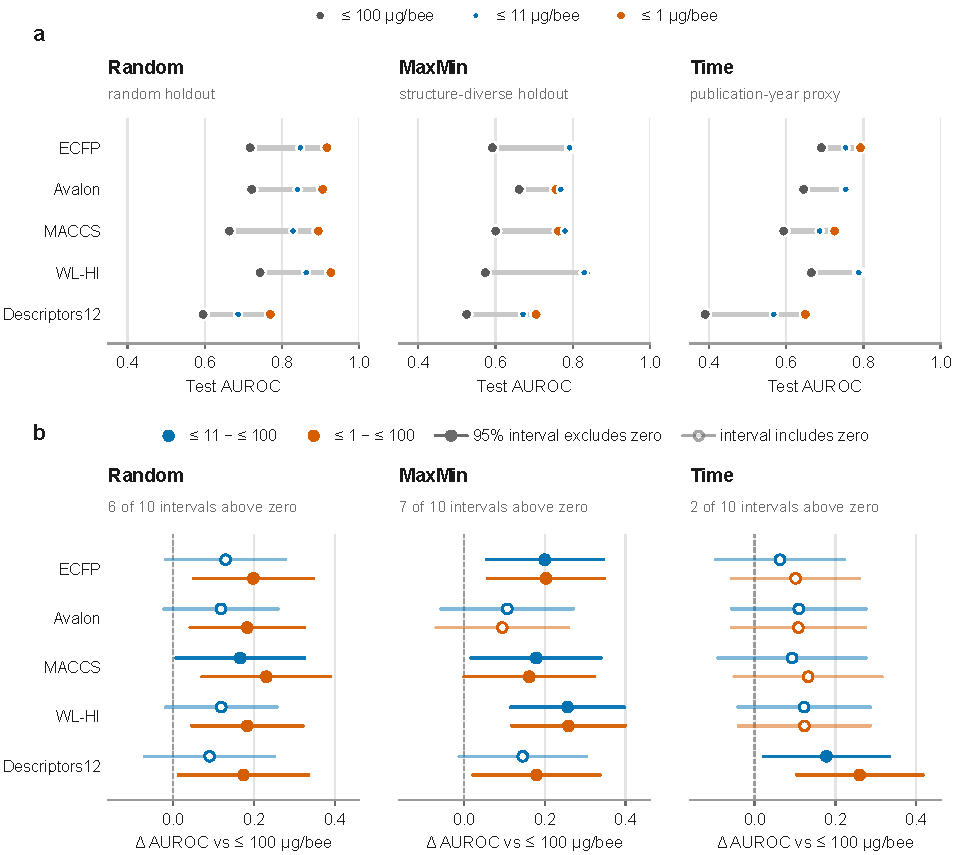
\includegraphics[width=\linewidth]{Fig2_endpoint_discriminability.pdf}
	\caption{\textbf{Endpoint definition changes measured discrimination.} \textbf{(a)} Test AUROC for five molecular representations under each official split; connectors span the three nested endpoints. \textbf{(b)} Paired endpoint contrasts with simultaneous 95\% confidence intervals from scaffold-cluster resampling. Filled markers denote intervals excluding zero. Intervals are simultaneous within each representation--split pair of endpoint contrasts. All 30 contrasts are positive, and 15 intervals exclude zero. Supplementary Table~S3 reports the ten-contrast sensitivity analysis.}
	\label{fig:performance}
\end{figure*}

\section{Results}
\subsection{The broad endpoint had lower discrimination on the released benchmark}
The 100~\ugbee endpoint had the lowest AUROC in all 15 representation--split settings (Fig.~\ref{fig:performance}a; Supplementary Table~S1 and Fig.~S1). Under MaxMin, ECFP AUROCs were 0.592, 0.792 and 0.795 at 100, 11 and 1~\ugbee. The severe-minus-broad differences were 0.200 and 0.203, with simultaneous scaffold-cluster 95\% intervals of 0.056--0.345 and 0.059--0.348 (Table~\ref{tab:contrasts}). Random differences were 0.130 and 0.199, with the primary interval excluding zero only for the latter; Time differences were 0.063 and 0.101, with both intervals spanning zero.

All 30 endpoint contrasts were positive in direction. Fifteen scaffold-cluster intervals excluded zero in the two-contrast family and seven in the ten-contrast family (Supplementary Tables~S2 and S3). Both MaxMin contrasts for ECFP and WL-HI retained support in the wider family. The broad endpoint was also lowest in all six additional logistic-regression and random-forest settings (Supplementary Table~S4). 

\begin{table*}[!t]
	\centering
	\caption{\textbf{Primary AUROC contrasts under structure-diverse evaluation.}}
	\label{tab:contrasts}
	\begin{threeparttable}
		\begin{tabularx}{\linewidth}{lYcc}
			\toprule
			\textbf{Resampling unit} &
			\textbf{Contrast} &
			$\boldsymbol{\Delta}$\textbf{AUROC} &
			\textbf{Simultaneous 95\% CI} \\
			\midrule
			Molecule & 11 versus 100 & 0.200 & 0.053 to 0.347 \\
			Molecule & 1 versus 100 & 0.203 & 0.056 to 0.350 \\
			Scaffold cluster & 11 versus 100 & \textbf{0.200} & \textbf{0.056 to 0.345} \\
			Scaffold cluster & 1 versus 100 & \textbf{0.203} & \textbf{0.059 to 0.348} \\
			\bottomrule
		\end{tabularx}
		\begin{tablenotes}[flushleft]\footnotesize
			\item Results correspond to the MaxMin split using the ECFP/Tanimoto support-vector machine, the primary structural probe. AUROC differences are defined as the more severe endpoint minus the 100~\ugbee endpoint. The joint centred bootstrap intervals describe reweighting variability in the current MaxMin test cohort, conditional on the fitted models, label rules and analysis protocol. Boldface denotes the scaffold-cluster inference. Complete bootstrap contrasts for all representations and splits are given in Supplementary Table~S2.
		\end{tablenotes}
	\end{threeparttable}
\end{table*}

\begin{figure*}[!t]
\centering
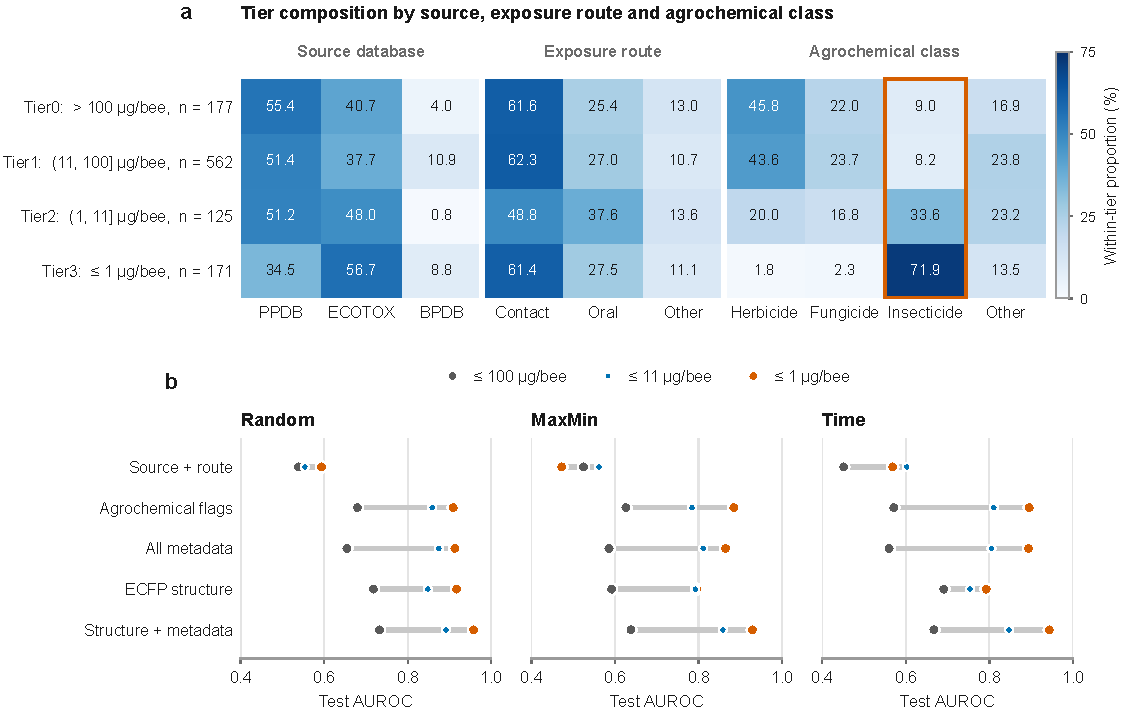
\includegraphics[width=\linewidth]{Fig3_composition_and_models.pdf}
\caption{\textbf{Chemical-use composition and model decomposition.} \textbf{(a)} Within-tier proportions for source database, exposure route and agrochemical class. The boxed column marks insecticide enrichment in the severe tiers; shares are 9.0\%, 8.2\%, 33.6\% and 71.9\% from Tier0 to Tier3. \textbf{(b)} Test AUROC for the source-plus-route, agrochemical-use and all-metadata models, the ECFP structure model and the out-of-fold fused model. Severe-endpoint discrimination is partly reproducible from non-structural metadata.}
\label{fig:composition}
\end{figure*}

\subsection{Chemical-use composition predicted the severe labels}
The four tiers contained 177, 562, 125 and 171 compounds. Insecticide shares were 9.0\%, 8.2\%, 33.6\% and 71.9\%, respectively, giving a tier--insecticide association of \(V=0.572\) (Fig.~\ref{fig:composition}a). Use-only models reached severe-endpoint AUROCs of 0.784--0.909 (Fig.~\ref{fig:composition}b; Supplementary Table~S5 and Fig.~S2). All-metadata MaxMin values were 0.811 and 0.865 at 11 and 1~\ugbee, compared with ECFP values of 0.792 and 0.795. Severe-label predictability was therefore present in both structure and chemical-use information.

Fusion exceeded metadata in 9/9 point comparisons and structure in 8/9, with the 100~\ugbee Time task as the exception. Matched preprocessing retained these counts (Supplementary Table~S6). With the original preprocessing, simultaneous intervals for fusion gains over metadata included zero; the clearest gain over structure occurred at 1~\ugbee under Time. These estimates characterize complementary prediction under the observed composition.

\subsection{Tier0--Tier1 comparisons accounted for much of the broad-endpoint deficit}
Tier1--Tier0 pairs formed 67\%, 74\% and 75\% of the broad endpoint's positive--negative comparisons in Random, MaxMin and Time. The broad ECFP model ranked these pairs with AUROCs of 0.676, 0.574 and 0.678, compared with 0.844, 0.668 and 0.805 for Tier3--Tier0 (Fig.~\ref{fig:tier-boundary}b; Supplementary Table~S11). Severe-trained scores also ranked Tier1 weakly relative to Tier0 under MaxMin (0.411 and 0.428) and Time (0.492 and 0.539). Under MaxMin, their AUROCs against the broad labels were 0.500--0.501 (Supplementary Table~S12). Thus, good discrimination of severe labels did not transfer to the comparisons dominating the broad task.

Equalizing training class counts retained the broad-endpoint disadvantage at every evaluated sample size in all three splits (Fig.~\ref{fig:tier-boundary}a; Supplementary Table~S9). At 125 compounds per class, MaxMin mean AUROCs were 0.554, 0.715 and 0.747. Source-holdout results retained the same direction, with wider uncertainty for BPDB (Supplementary Table~S10).

\begin{figure*}[!t]
\centering
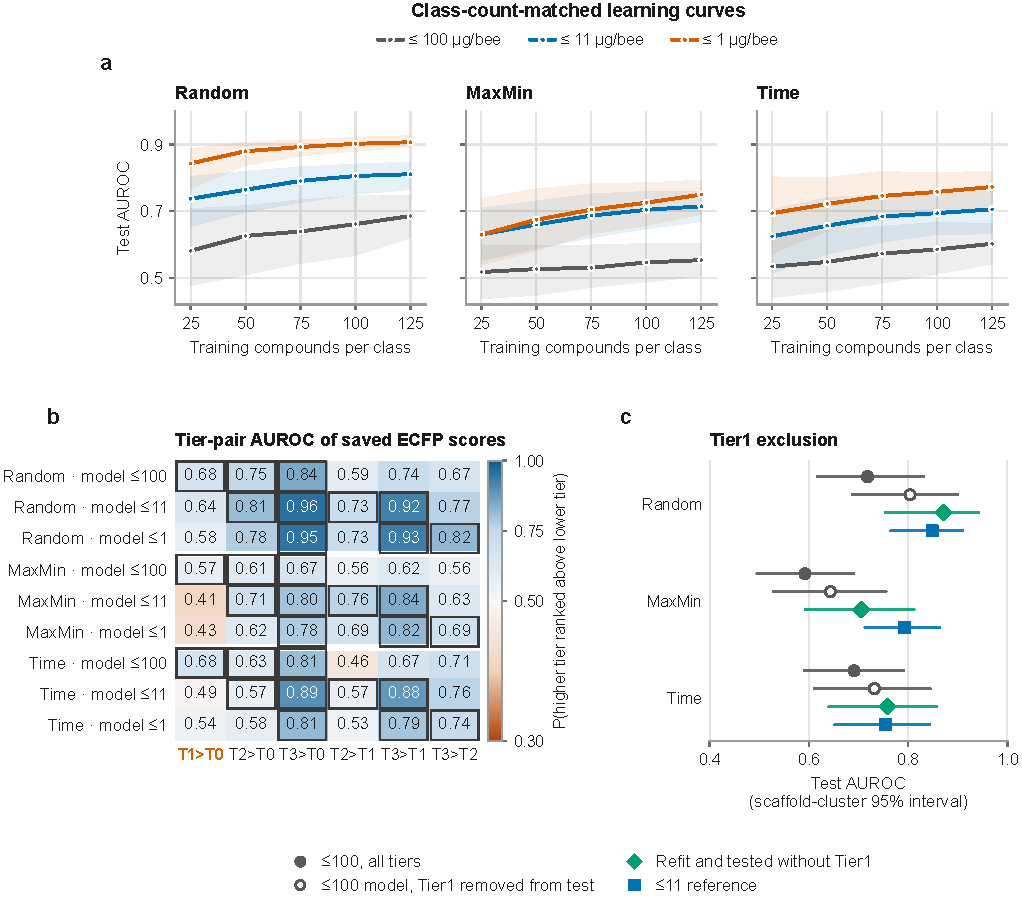
\includegraphics[width=0.98\linewidth]{Fig4_class_count_and_tier_boundary.pdf}
\caption{\textbf{The broad-endpoint deficit survives class-count matching and is concentrated at the Tier0/Tier1 boundary.} \textbf{(a)} Class-count-matched learning curves; lines are medians and bands are 2.5--97.5\% ranges over 200 balanced training subsamples. \textbf{(b)} Tier-pair AUROC of the saved ECFP test scores for the model trained at each endpoint. Each cell is the probability that a compound of the higher tier outranks one of the lower tier; outlined cells enter that model's own endpoint AUROC through \eqref{eq:tier-pair}. \textbf{(c)} Tier1 exclusion: the broad model on all test tiers, the same model with Tier1 removed from the test set, the model refitted and tested without Tier1, and the 11~\ugbee endpoint as reference. Bars are scaffold-cluster 95\% percentile intervals.}
\label{fig:tier-boundary}
\end{figure*}

Removing Tier1 from evaluation increased the broad-model AUROC from 0.718 to 0.804 under Random, from 0.592 to 0.643 under MaxMin and from 0.691 to 0.732 under Time. Refitting without Tier1 increased these values to 0.871, 0.705 and 0.758 (Fig.~\ref{fig:tier-boundary}c; Table~\ref{tab:tier1}). Under MaxMin, the deletion component was 0.113 of the original 0.200 gap, leaving 0.087 (95\% interval 0.012--0.166). Across representations, the component was positive in 15/15 settings and had a scaffold-cluster interval above zero in 8 (Supplementary Table~S14). 

\begin{table*}[!t]
\centering
\caption{\textbf{Tier1 exclusion and the broad-endpoint AUROC gap (ECFP).}}
\label{tab:tier1}
\begin{threeparttable}
\footnotesize
\begin{tabularx}{\linewidth}{l*{4}{>{\centering\arraybackslash\hsize=0.78\hsize}X}c*{2}{>{\centering\arraybackslash\hsize=1.44\hsize}X}}
\toprule
\textbf{Split} & {\bfseries $\leq$100, all tiers} & {\bfseries $\leq$100 model, Tier1 removed from test} & \textbf{Refit and tested without Tier1} & {\bfseries $\leq$11, all tiers} & \textbf{Gap} & \textbf{Tier1 component (95\% CI)} & \textbf{Residual (95\% CI)} \\
\midrule
Random & 0.718 & 0.804 & 0.871 & 0.848 & 0.130 & 0.153 (0.023 to 0.242) & $-$0.023 ($-$0.081 to 0.058) \\
MaxMin & 0.592 & 0.643 & 0.705 & 0.792 & 0.200 & 0.113 (0.017 to 0.212) & 0.087 (0.012 to 0.166) \\
Time & 0.691 & 0.732 & 0.758 & 0.754 & 0.063 & 0.067 ($-$0.048 to 0.183) & $-$0.004 ($-$0.083 to 0.078) \\
\bottomrule
\end{tabularx}
\begin{tablenotes}[flushleft]\footnotesize
\item Test AUROC of the ECFP/Tanimoto SVM. Gap: \(\leq11\) minus \(\leq100\) on all test tiers. Tier1 component: refit without Tier1 minus \(\leq100\) on all tiers; residual: \(\leq11\) minus the refit. The components add to the gap (Eq.~\eqref{eq:tier1-decomposition}). Intervals are scaffold-cluster 95\% percentile intervals over the primary bootstrap draws. Without Tier1, the two cut-offs define the same labels on the reduced set; the all-tier 11~\ugbee reference still uses its original train/test members. All representations are given in Supplementary Table~S14.
\end{tablenotes}
\end{threeparttable}
\end{table*}

\subsection{Upstream reconstruction separated qualifier loss from aggregation choices}
The upstream ApisTox code reproduced all 441 ECOTOX-derived binary labels, ternary levels and determining routes. It also confirmed a specific processing defect: omitting the operator makes a \(>100\)~\ugbee response enter the ternary rule as exactly 100\cite{ApisToxCode}. Of 212 ECOTOX-derived Tier1 compounds, 180 (84.9\%) had a right-censored record in the determining group.

With those historical groups fixed, numerical-median rule A gave 212 positive labels at 100~\ugbee, whereas numerical-consensus rule B gave 195 positive and 17 unresolved labels. Restoring qualifiers under consensus rule C gave 32 positive, 67 negative and 113 unresolved labels; interval-median rule D gave 37, 69 and 106, respectively (Fig.~\ref{fig:provenance}b; Supplementary Tables~S17 and S22). The change from A to C therefore includes both qualifier restoration and a change in aggregation. The unresolved category retained information that neither binary label could express.

\begin{figure*}[!t]
\centering
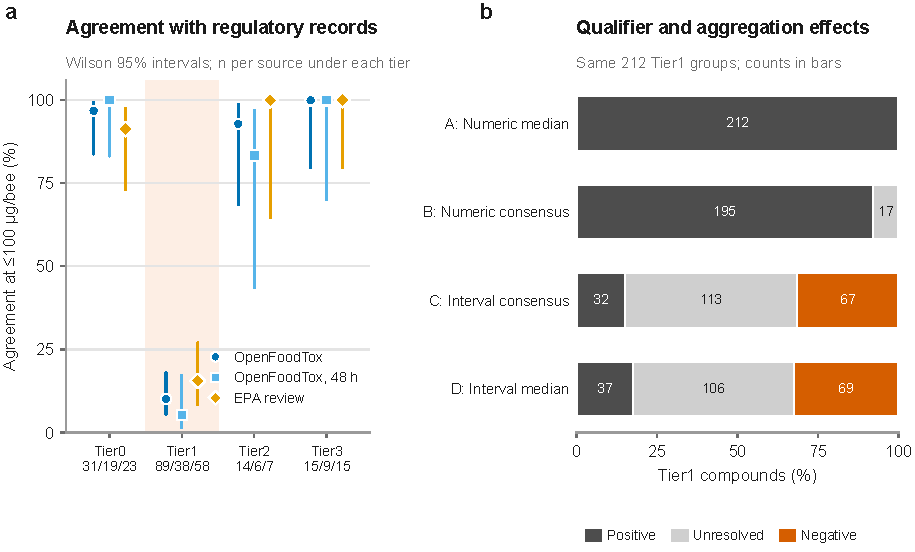
\includegraphics[width=\linewidth]{Fig5_label_provenance.pdf}
\caption{\textbf{Regulatory disagreement and aggregation-dependent label changes.} \textbf{(a)} Agreement between benchmark labels and route-matched regulatory labels at 100~\ugbee, by benchmark tier, with Wilson 95\% intervals; numbers beneath each tier give the cohort sizes for OpenFoodTox, its 48-hour/material-field screen and the EPA retrospective. \textbf{(b)} Positive, unresolved and negative labels for the 212 ECOTOX-derived Tier1 compounds under four rules applied to the same historical determining groups: A, numerical median; B, numerical consensus; C, qualifier-aware consensus; D, qualifier-aware interval median. All records must be determinate and agree under consensus. Unresolved denotes threshold-ambiguous intervals or, for consensus, disagreement among records. The A-to-C change therefore includes both qualifier handling and aggregation.}
\label{fig:provenance}
\end{figure*}

The determining groups differed in life stage, duration and dose basis. Among the 441 determining groups, 316 contained only adult records, 276 only exact 48-hour records, and 43 included daily-dose units. Within the 146 Tier1 groups consisting entirely of adult, 48-hour, non-daily-dose observations, rule C gave 16 positive, 60 negative and 70 unresolved labels. At the severe cut-off, 17 of 157 originally positive ECOTOX labels at 11~\ugbee became unresolved under rule C. The Tier3 compound with Chemical Abstracts Service (CAS) number 115970-17-7 had three records reported as \(>1000\) ng/organism, equivalent to \(>1\)~\ugbee (Supplementary Tables~S22 and S24).

Separately curated regulatory records showed concentrated disagreement with Tier1 annotations. On same-route cohorts with all three labels determined, OpenFoodTox disagreed with the benchmark for 2/149, 1/149 and 82/149 compounds at 1, 11 and 100~\ugbee; EPA counts were 2/103, 3/103 and 51/103 (Supplementary Table~S15). At 100~\ugbee, Tier1 agreement was 9/89 for OpenFoodTox, 2/38 after its 48-hour/material-field screen and 9/58 for EPA (Fig.~\ref{fig:provenance}a; Table~\ref{tab:concordance}). Every Tier1 disagreement changed a benchmark-positive to a source-negative label, and \(>100\) evidence accounted for 70/80, 30/36 and 39/49 disagreements, respectively. These proportions describe the selected source cohorts; study-level correspondence remains incomplete.

\begin{table}[!t]
\centering
\caption{\textbf{Agreement at 100~\ugbee between benchmark tiers and route-matched regulatory labels.}}
\label{tab:concordance}
\begin{tabularx}{\linewidth}{lCCC}
\toprule
\textbf{Tier} & \textbf{OFT} & \textbf{OFT, 48 h} & \textbf{EPA} \\
\midrule
Tier0 & 30/31 (96.8) & 19/19 (100.0) & 21/23 (91.3) \\
Tier1 & 9/89 (10.1) & 2/38 (5.3) & 9/58 (15.5) \\
Tier2 & 13/14 (92.9) & 5/6 (83.3) & 7/7 (100.0) \\
Tier3 & 15/15 (100.0) & 9/9 (100.0) & 15/15 (100.0) \\
\bottomrule
\end{tabularx}
\vspace{2pt}
\parbox{\linewidth}{\footnotesize Agreeing compounds/compounds (\%) in same-route cohorts with all three source labels determined. OFT: OpenFoodTox; OFT, 48 h: 48-hour observations without material-review flags or explicit test-material dose reports; EPA: the 2022 EPA retrospective. All Tier1 disagreements had a benchmark label at or below 100~\ugbee and a source label above it. Wilson intervals and record-source counts are given in Supplementary Table~S16.}
\end{table}

\begin{figure*}[!t]
\centering
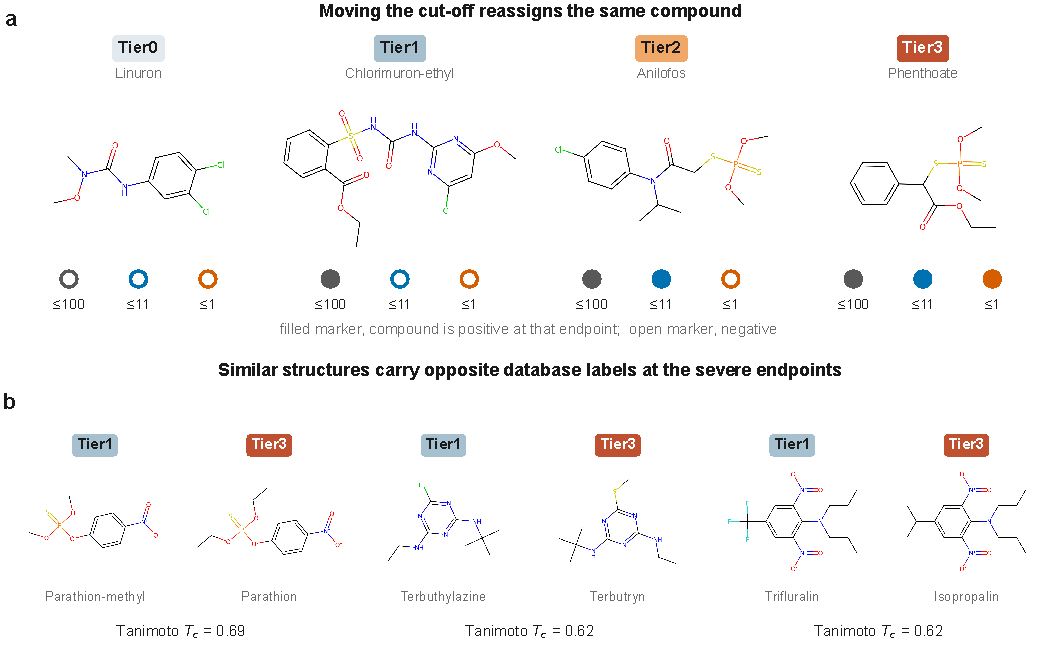
\includegraphics[width=\linewidth]{Fig6_chemical_structures.pdf}
\caption{\textbf{Chemical structures behind the endpoint definitions.} \textbf{(a)} Medoid compound of each analytical tier in ECFP space, with class membership at each nested endpoint; filled markers denote positive and open markers negative. \textbf{(b)} Three pairs selected greedily by decreasing ECFP4 Tanimoto similarity from shared-scaffold Tier0/1--Tier3 candidates, without reusing a compound. All displayed pairs carry Tier1--Tier3 labels.}
\label{fig:structures}
\end{figure*}

\begin{figure*}[!t]
\centering
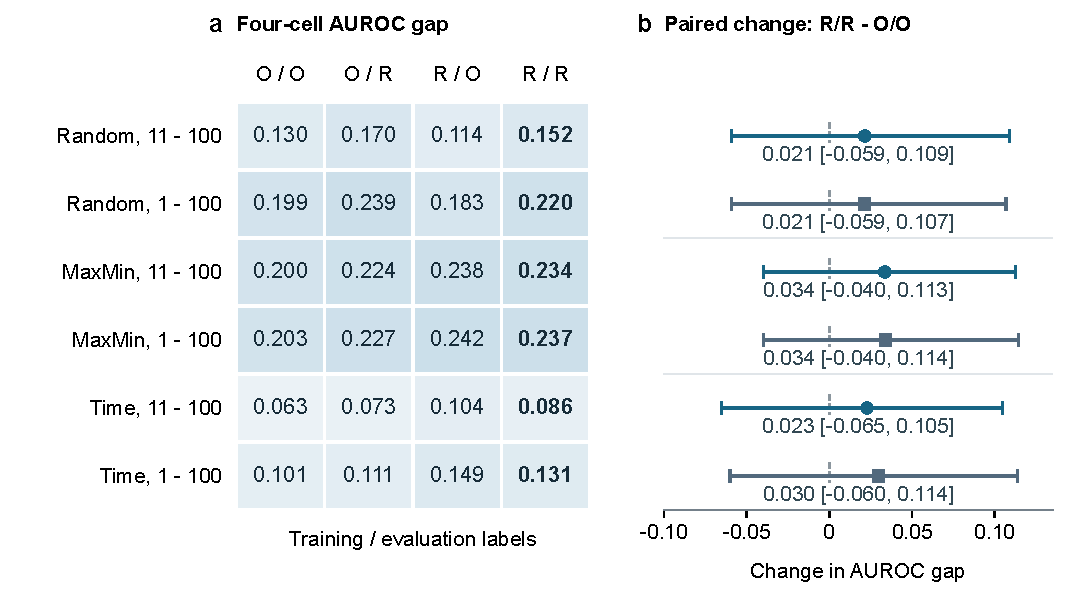
\includegraphics[width=\linewidth]{Fig7_label_crossover.pdf}
\caption{\textbf{Matched-cohort provisional revisions and endpoint discrimination gaps.} \textbf{(a)} ECFP severe-minus-broad AUROC differences for all four combinations of original (O) and provisionally revised (R) training and evaluation labels, for each official split and both severe cut-offs. The first and second letters denote training and evaluation label versions, respectively; O and R are distinct from aggregation rules A--D. \textbf{(b)} The paired change after provisionally revising both training and evaluation labels (R/R minus O/O), with conditional 95\% percentile intervals from 2,000 shared scaffold-cluster draws. Positive values mean a wider gap. The primary revision uses qualifier-aware interval medians at 1 and 100~\ugbee and consensus at 11~\ugbee over upstream-eligible ECOTOX routes. Unresolved labels retain their original values; all cells use the same 828 training and 207 test identities within each split. Broad-endpoint test labels changed for 15, 12 and 19 compounds under Random, MaxMin and Time, respectively. Intervals describe within-cohort reweighting under fixed models, label rules and analysis protocol, without adjustment across revision scenarios. Differences are calculated before rounding. Complete results are in Supplementary Table~S23.}
\label{fig:crossover}
\end{figure*}

Illustrative structures identify a discrepancy in the opposite direction (Fig.~\ref{fig:structures}). The three highest-ranked non-overlapping pairs selected greedily from 3,421 shared-scaffold Tier0/1--Tier3 candidates were methyl parathion/parathion, terbuthylazine/terbutryn and trifluralin/isopropalin, with ECFP similarities of 0.69, 0.62 and 0.62. Methyl parathion carries a Tier1 annotation, whereas EPA reports a 48-hour technical-material contact LD\(_{50}\) of 0.291~\ugbee (MRID 00022220)\cite{EPAMethylAssessment}, which would place that contact observation in Tier3. Methyl parathion therefore illustrates a cross-source label disagreement with unmatched historical study identity. The other two pairs provide structural context.

Source-label reassessment on training-excluded regulatory cohorts changed saved-score AUROCs in both directions. The small cohorts and their class counts are reported in Supplementary Tables~S18a--b and Fig.~S4.

\subsection{Matched-cohort provisional revisions did not consistently narrow the gap}
The crossover compared original and provisionally revised training and evaluation labels on identical members (Fig.~\ref{fig:crossover}). With unresolved labels retained, the primary revision changed 69, 0 and 1 compound labels at 100, 11 and 1~\ugbee, respectively. The 11~\ugbee labels were unchanged in both training and test sets. Under this scenario, the ECFP 11-minus-100 gap changed from 0.130 to 0.152 under Random, from 0.200 to 0.234 under MaxMin and from 0.063 to 0.086 under Time when both training and evaluation labels were provisionally revised. The 1-minus-100 changes were also positive in point estimate. The MaxMin 11-minus-100 change was 0.034 (95\% interval $-$0.040 to 0.113). All six intervals for the paired changes spanned zero (Fig.~\ref{fig:crossover}b).

Under MaxMin, the broad-endpoint AUROC changed from 0.592 to 0.568 after provisionally revising evaluation labels and to 0.558 after provisionally revising both training and evaluation labels. Other scenarios and representations produced changes in both directions, without consistent evidence of gap reduction (Supplementary Table~S23). The crossovers estimate the effect of the specified, identifiable revisions; retaining unresolved labels leaves part of the original annotation uncertainty in the partially revised benchmark.

The aggregation sensitivity gave identical final labels under keep when rule D replaced consensus at 11~\ugbee. Under exclude, all-D retained two additional identities; all paired gap-change intervals still spanned zero (Supplementary Table~S25). Excluding the 33 current identifier-screening cases also retained the broad-endpoint disadvantage in all three ECFP splits; MaxMin AUROCs were 0.587, 0.799 and 0.796 (Supplementary Table~S26).





\subsection{Unseen-identity cases distinguished ranking from default decisions}
Six identities supplied eleven eligible 48-hour endpoints: acynonapyr, cyclobutrifluram, flupentiofenox, fluxametamide, isocycloseram and spiropidion (Supplementary Tables~S19a--b). The contact cohort contained one compound in \((1,11]\) and four above 100~\ugbee, so its 1~\ugbee AUROC was undefined and its 11 and 100~\ugbee labels were identical. Contact AUROC under Random was 0.75 at 11 and 1.00 at 100~\ugbee (1.00 and 0.75, respectively, under MaxMin and Time), yet every 11~\ugbee model missed fluxametamide at the zero-score boundary. The four-compound common oral cohort likewise had identical labels across cut-offs, and every 1 and 11~\ugbee model missed its two positives (Supplementary Table~S20). The six-identity case study illustrates how ranking and default-decision outcomes differ within the represented tiers.

\section{Discussion}
This audit connects the observed endpoint gap in ApisTox to the comparisons and processing rules that define its tasks. Tier-pair analysis identifies the weakly ranked Tier1--Tier0 boundary, while upstream replay verifies qualifier loss within the historical determining records. Matched-cohort revision tests then show that provisionally revising identifiable labels does not consistently narrow the gap. These results distinguish the fidelity of a benchmark annotation from the discrimination achieved against it.

The broad endpoint placed most of its positive--negative comparisons at the weakly ranked Tier1--Tier0 boundary. Tier1 deletion locates these comparisons but also changes the populations on which models are trained and tested. The crossover holds those identities fixed and instead changes the labels. Its intervals permit both decreases and increases in the gap, while unresolved records limit the extent of correction. Together with the chemical-use composition differences, these results leave the causal contribution of annotation errors to the original gap undetermined.

Prior honey-bee models have screened assay conditions, reconciled repeated observations and retained qualifiers\cite{Carnesecchi2020,Iovine2026}; QSAR studies have also compared alternative threshold schemes\cite{Wang2023}. The present contribution traces a released benchmark's labels back through its processing rules and tests their predictive consequences on matched cohorts. The combination makes both the record-to-label transformation and the predictive effect of its revision inspectable, extending explicit endpoint and aggregation specifications\cite{Nael2026} into a reproducible evaluation. The factorial audit makes one distinction particularly clear: changing from medians to all-record consensus can alter labels before any inequality operator is restored. Qualifier-aware aggregation must therefore state both the numerical rule and how ambiguous or conflicting records are represented. Converting \(>100\) to 100 preserves the 11~\ugbee label for that observation, although other bounds and the route-selection rule can affect severe labels.

ECOTOX groups mix life stages, durations and dose bases; historical PPDB/BPDB input snapshots remain unavailable. Current identifier checks revealed source-specific inconsistencies, but the historical PubChem responses needed to reconstruct individual year assignments were not preserved. The identifier-exclusion sensitivity tests their screening set, not a corrected chronology. Regulatory comparisons cover selected pesticide subsets and may share underlying studies with the benchmark, so they cannot establish a benchmark-wide error rate. Earlier inspection of the official test sets also makes the performance analysis retrospective, and the reported intervals condition on fitted models.

The unseen-identity cases show why ranking and default classification need separate assessment. An AUROC above chance did not ensure detection at the balanced SVM's zero-score boundary. These case-level differences motivate evaluating explicit decision thresholds alongside ranking metrics when the intended use is chemical screening. A larger cohort with harmonized observations and multiple represented tiers would be needed to evaluate that use.

Future validation with independently adjudicated records and newly held-out compounds can assess how more complete label correction changes generalization. A benchmark release can make these distinctions inspectable by preserving qualified source values, eligibility filters, aggregation rules and unresolved outcomes alongside the labels. Tier-pair AUROCs then identify which comparisons determine each endpoint's score, and matched-cohort crossovers test the effects of a specified correction.

\section{Conclusion}
This audit characterizes endpoint-dependent discrimination and label construction in ApisTox. The broad 100~\ugbee endpoint had the lowest AUROC across the five evaluated representations and three official splits under the specified SVM protocols. The deficit was concentrated in Tier1--Tier0 comparisons. Source and code audits confirmed qualifier loss, while identifiable provisional revisions produced no consistent narrowing of the gap. Preserving source qualifiers and evaluating revisions on matched cohorts are complementary requirements for interpretable toxicity benchmarking.

\section*{Acknowledgment}
The authors thank the creators and maintainers of ApisTox for making the dataset and its construction code publicly available. The authors also thank the Data Science Innovation and Entrepreneurship Laboratory at Hanshan Normal University for providing computational resources and research support.
OpenAI Codex (\url{https://openai.com/codex/}) assisted with drafting the literature comparison in Section~II-C, clarifying the generalized estimating equation assumptions in the Supplementary Information, and language editing.

\section*{Data Availability}
ApisTox v2 is available at \url{https://doi.org/10.5281/zenodo.13350981}\cite{Adamczyk2025}, and OpenFoodTox 3.0 v7 at \url{https://doi.org/10.5281/zenodo.19388272}\cite{OFT2026}. The EPA retrospective tables accompany their source publication\cite{Farruggia2022}. Input data, split memberships, processed labels, saved predictions and source-record ledgers are provided in the accompanying \textit{Research Materials} and the \href{https://github.com/hiiiy-pm/Endpoint-Definitions-and-Label-Provenance-in-Honey-Bee-Toxicity-Benchmarking/releases/latest}{study repository archive}. The source ledgers retain record identifiers and links to the underlying data.

\section*{Code Availability}
Analysis and figure-generation code, environment specifications and reproduction instructions are available in the \href{https://github.com/hiiiy-pm/Endpoint-Definitions-and-Label-Provenance-in-Honey-Bee-Toxicity-Benchmarking}{GitHub repository} and accompanying \textit{Research Materials}. The \texttt{LaTeX\_Source.zip} archive contains the manuscript and Supplementary Information sources, bibliography, figure assets and build script. Cached upstream ApisTox code is pinned to commit 57c2c05\cite{ApisToxCode}. Study code uses the MIT License; third-party data retain their original terms.

\section*{Ethics Statement}
This study is a secondary computational analysis of public chemical and ecotoxicological data. It involved no human participants, personal data or new animal experiments.

\section*{Conflict of Interest}
The authors declare no conflict of interest.

\bibliographystyle{IEEEtran}
\bibliography{references}

% Keep the three biographies together in the final right column.
\newpage

\begin{IEEEbiography}[{
\includegraphics[width=1in,height=1.25in,keepaspectratio]{author_photos/yongye_huang.jpg}}]{Yongye Huang}
is currently pursuing the B.S. degree in Data Science and Big Data Technology with the School of Mathematics and Statistics, Hanshan Normal University, Chaozhou, China. His research interests include machine learning, data quality in benchmark datasets, and computational toxicology.
\end{IEEEbiography}

\begin{IEEEbiography}[{
\includegraphics[width=1in,height=1.25in,keepaspectratio]{author_photos/runqing_liao.jpg}}]{Runqing Liao}
is currently pursuing the B.S. degree in Data Science and Big Data Technology with the School of Mathematics and Statistics, Hanshan Normal University, Chaozhou, China. His research interests include machine learning, deep learning, medical data analysis, and medical image analysis.
\end{IEEEbiography}

\begin{IEEEbiography}[{
\includegraphics[width=1in,height=1.25in,keepaspectratio]{author_photos/zhining_wang.jpg}}]{Zhining Wang}
received the M.S. degree from South China Normal University, Guangzhou, China. He is currently a Lecturer with the School of Mathematics and Statistics, Hanshan Normal University, Chaozhou, China. His research interests include statistical inference, applied mathematical modeling, machine learning, and artificial intelligence.
\end{IEEEbiography}

\EOD

\end{document}
